\documentclass[12pt]{article}
\usepackage{times}
\usepackage{latexsym}
\usepackage{graphicx}
\usepackage{url}
\usepackage{float}

\linespread{1}
\title{Anthropocentric Bias in Viral Genome Sequencing: Which Viruses Get Sequenced?}
\date{\today}
\author{Jacob Osborne}


\begin{document}

    \begin{titlepage}
        \begin{center}
            \vspace*{1in}
            \LARGE
            Anthropocentric Bias in Viral Genome Sequencing: Which Viruses Get Sequenced?

            \vspace*{1in}
            \large
            Jacob Osborne

            \vfill
            [DEGREE PROGRAM] \\
            Dr. Claus Wilke, Integrative Biology \\
            \today
        \end{center}
    \end{titlepage}
    
    \begin{abstract}
        PLACEHOLDER TEXT PLEASE IGNORE
    \end{abstract}

    \section{Introduction}

    The NCBI Viral Genomes database provides a large catalogue of viral genomes 
    sequenced by scientists around the world. It is the preeminent resource for
    obtaining records of viral genomes for scientific analysis. \\
    Yet, there is some doubt as to the extent to which the genomes catalogued
    therein can be taken as representative of viral genomes present in the
    natural world as a whole. We suspect the genomes of viruses that infect
    humans, domestic animals, and domestic plants - living things that are
    directly relevant to human life - are far more likely to be sequenced than
    the genomes of those which do not. \\
    The aim of this project, therefore, is to ascertain the extent of this
    anthropocentric bias in the NCBI database.

    \section{Data}

    The NCBI viral genomes database does not provide information on the hosts
    of the viruses it contains records on. Thankfully, the Virus-Host Database provides
    linkages between the various NCBI databases' (including the Viral Genomes
    database) records for viruses and the records for their hosts. Therefore,
    this project uses data from the Viral-Host Database instead of the NCBI viral
    genomes database directly. \\
    The Virus-Host Database in its entirety - 14,042 unique records - is utilized in
    this project. \\
    This presents a difficulty, however - the Virus-Host Database's records are formatted
    as a relationship between a single virus and a single piece of literature
    that shows at least one host for that virus, with the hosts shown in that
    literature linked by the record, rather than as a relationship between a
    virus and its hosts. \\
    Therefore, much of the code in the project is dedicated to transforming
    the format of the data contained within into a one-to-many relationship
    of viruses to their hosts.

    %\section{Methodology}
    
    %Data obtained from the Virus-Host Database was reformatted into a "one Virus
    %to many Hosts" format using a python script, the code for which is presented
    %in the Appendix. \\
    %From this data, a breakdown of the clades to which host species present in the
    %database belonged. Further, a breakdown of the number of viruses which infect
    %species of each clade was also obtained.

    \section{Preliminary Analysis}

    \begin{figure}[H]
        \begin{center}
            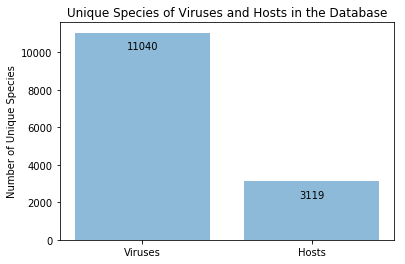
\includegraphics[width=100mm]{unique_species_figure.png}
            \caption{A comparison of the number of unique species of virus and of
            host present in the database.}
            \label{unique_species_figure}
        \end{center}
    \end{figure}

    As shown in Figure \ref{unique_species_figure}, there are just under 3
    times as many unique species of virus as of host. This means we can expect,
    for each host species in the database, multiple species of virus that infect
    it.
    

    \begin{figure}[H]
        \begin{center}
            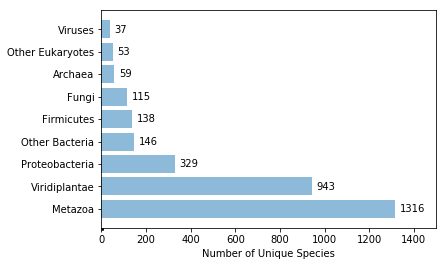
\includegraphics[width=120mm]{host_clades_figure.png}
            \caption{A breakdown of the kingdoms to which host species present in
            the database belong.}
            \label{host_clades_figure}
        \end{center}
    \end{figure}

    Figure \ref{host_clades_figure} shows the vast majority of host species in
    the database are either animals (Metazoa) or plants (Viridiplantae). Fungal
    host species are relatively uncommon in the data. We see a similar pattern
    in the clades viruses can infect:
    

\end{document}